\documentclass[12pt,a4paper]{report}

%% ── Packages ──────────────────────────────────────────────────────────────────
\usepackage[utf8]{inputenc}
\usepackage[T1]{fontenc}
\usepackage{lmodern}
\usepackage[margin=1in]{geometry}
\usepackage{graphicx}
\usepackage{float}
\usepackage{amsmath,amssymb}
\usepackage{algorithm}
\usepackage{algpseudocode}
\usepackage{booktabs}
\usepackage{multirow}
\usepackage{xcolor}
\usepackage{listings}
\usepackage{caption}
\usepackage{subcaption}
\usepackage{hyperref}
\usepackage{url}
\usepackage{cite}
\usepackage{setspace}
\usepackage{fancyhdr}
\usepackage{titlesec}
\usepackage{enumitem}
\usepackage{pgfplots}
\pgfplotsset{compat=1.18}
\usepackage{tikz}
\usetikzlibrary{shapes.geometric, arrows.meta, positioning, fit, backgrounds}

%% ── Formatting ────────────────────────────────────────────────────────────────
\onehalfspacing
\hypersetup{colorlinks=true, linkcolor=blue!70!black, citecolor=green!50!black, urlcolor=blue}

\pagestyle{fancy}
\fancyhf{}
\rhead{\small SplitFed Learning over Heterogeneous Networks}
\lhead{\small Undergraduate Thesis}
\cfoot{\thepage}

%% ── Code listing style ────────────────────────────────────────────────────────
\lstset{
  basicstyle=\ttfamily\footnotesize,
  breaklines=true,
  frame=single,
  backgroundcolor=\color{gray!8},
  keywordstyle=\color{blue!70!black}\bfseries,
  commentstyle=\color{green!50!black},
  stringstyle=\color{red!70!black},
  numbers=left,
  numberstyle=\tiny\color{gray},
  numbersep=8pt,
  captionpos=b
}

%% ─────────────────────────────────────────────────────────────────────────────
\begin{document}

%% ── Title Page ────────────────────────────────────────────────────────────────
\begin{titlepage}
  \centering
  \vspace*{1.5cm}
  {\LARGE\bfseries SplitFed Learning over Heterogeneous Networks:\\[0.4em]
  A QoS-Aware Analysis of TCP Throughput Constraints\\[0.4em]
  on Federated Model Convergence\par}
  \vspace{1.5cm}
  {\large Undergraduate Thesis\par}
  \vspace{0.5cm}
  {\large Department of Computer Science\par}
  \vspace{2cm}
  {\large\bfseries Student Name\par}
  \vspace{0.5cm}
  {\large Supervisor: Dr.\ Zubair Fadlullah\par}
  \vspace{2cm}
  {\large \today\par}
  \vfill
  {\small Submitted in partial fulfilment of the requirements for the\\
  Bachelor of Science in Computer Science}
\end{titlepage}

%% ── Abstract ──────────────────────────────────────────────────────────────────
\begin{abstract}
\addcontentsline{toc}{chapter}{Abstract}
Federated learning (FL) enables collaborative model training across distributed clients without sharing raw data, making it attractive for privacy-sensitive applications. SplitFed learning extends this paradigm by splitting the neural network between clients and a central server, reducing the computational burden on resource-constrained edge devices. However, existing SplitFed implementations are typically demonstrated under ideal network conditions, leaving unanswered the question of how real-world network impairments affect system performance and model convergence.

This thesis presents a Docker-based SplitFed learning framework evaluated under controlled network conditions using Linux traffic control (\texttt{tc netem}). A ResNet-18 model is trained on a heterogeneous, non-IID image classification task across three federated clients. Network Quality of Service (QoS) parameters—bandwidth, round-trip latency, and packet loss—are systematically varied to characterize their impact on per-round communication latency, total training time, model accuracy, and convergence behaviour. Results identify a minimum effective TCP throughput threshold below which FL round integrity degrades, and provide a quantitative model of the accuracy-versus-bandwidth tradeoff. Practical client selection guidelines are derived from these thresholds to support SplitFed deployment in bandwidth-constrained environments such as 5G edge, IoT, and distributed healthcare networks.
\end{abstract}

\tableofcontents
\listoffigures
\listoftables

%% ══════════════════════════════════════════════════════════════════════════════
\chapter{Introduction}
%% ══════════════════════════════════════════════════════════════════════════════

\section{Background and Motivation}

The proliferation of edge devices and growing concerns about data privacy have accelerated interest in distributed machine learning paradigms that keep sensitive data local. Federated Learning (FL), first proposed by McMahan et al.\ \cite{mcmahan2017communication}, allows a global model to be trained across many clients by aggregating locally computed model updates rather than raw data. Despite its privacy advantages, classical FL places a significant computational burden on clients that must perform a full forward and backward pass over a potentially large neural network.

Split Learning (SL) \cite{gupta2018distributed} addresses this by partitioning a deep network at a designated \emph{cut layer}: the client processes only the shallow layers and transmits intermediate activations (the \emph{smashed data}) to the server, which handles the deeper layers and backpropagation. SplitFed Learning (SFL) \cite{thapa2022splitfed} combines both paradigms—clients train their portion of the network in parallel (federation) while offloading the compute-heavy upper layers to the server (splitting).

A critical but underexplored aspect of SplitFed deployment is the sensitivity of the training process to network conditions. Every FL round requires each client to: (i) download the current global model (or cut-layer weights), (ii) perform local training, and (iii) upload model updates. In heterogeneous networks—such as those comprising mobile devices, IoT sensors, and hospital workstations—clients may have vastly different available bandwidth, latency, and packet loss characteristics. The impact of these variations on convergence speed and final model accuracy is the central question of this thesis.

\section{Problem Statement}

Existing SplitFed implementations are validated primarily under ideal, local network conditions (e.g., Docker bridge networks on a single machine) that provide effectively unlimited bandwidth and near-zero latency. This leaves open a fundamental practical question:

\begin{quote}
\emph{What is the minimum TCP throughput a federated client requires to participate usefully in a SplitFed training process, and how do bandwidth, latency, and packet loss jointly affect convergence rate and final model accuracy under a non-IID data distribution?}
\end{quote}

Answering this question has direct implications for: client selection policies in FL systems; resource allocation in 5G and beyond-5G (B5G) edge networks; and the feasibility of deploying SplitFed in bandwidth-limited domains such as rural healthcare or industrial IoT.

\section{Objectives}

The specific objectives of this thesis are:
\begin{enumerate}[label=\textbf{O\arabic*.}]
  \item Design and implement a reproducible Docker-based SplitFed learning testbed with programmable network impairment injection.
  \item Characterise per-round communication cost (payload size, transfer latency) as a function of model architecture and cut-layer choice.
  \item Conduct a systematic QoS parameter sweep (bandwidth, RTT, packet loss) and measure the effect on convergence rounds, per-round duration, and final accuracy.
  \item Derive a minimum effective bandwidth threshold and an accuracy-versus-bandwidth degradation model.
  \item Propose a network-aware client selection heuristic for SplitFed deployments.
\end{enumerate}

\section{Contributions}

The main contributions of this work are:
\begin{itemize}
  \item A fully reproducible, open-source Docker Compose SplitFed testbed with integrated \texttt{tc netem} network emulation (Section~\ref{sec:impl}).
  \item Empirical characterisation of SplitFed communication cost on ResNet-18 under non-IID heterogeneous data (Section~\ref{sec:qos}).
  \item A quantitative throughput-convergence model identifying the bandwidth floor for stable FL training (Section~\ref{sec:results}).
  \item A network-aware client admission criterion applicable to 5G edge and IoT SplitFed deployments (Section~\ref{sec:future}).
\end{itemize}

\section{Thesis Structure}

Chapter~\ref{ch:related} surveys related work in FL, SL, and network-aware ML. Chapter~\ref{ch:problem} formalises the problem. Chapter~\ref{ch:method} describes the SplitFed architecture and experimental methodology. Chapter~\ref{ch:impl} details the software implementation. Chapter~\ref{ch:qos} presents the QoS analysis and experimental results. Chapter~\ref{ch:future} discusses future research directions. Chapter~\ref{ch:conclusion} concludes the thesis.

%% ══════════════════════════════════════════════════════════════════════════════
\chapter{Related Work}
\label{ch:related}
%% ══════════════════════════════════════════════════════════════════════════════

\section{Federated Learning}

McMahan et al.\ \cite{mcmahan2017communication} introduced the FedAvg algorithm, which remains the dominant FL aggregation scheme. FedAvg aggregates client model updates as a weighted average proportional to local dataset size. Subsequent work has addressed statistical heterogeneity (non-IID data) \cite{li2020federated}, communication efficiency \cite{konevcny2016federated}, and client selection under system heterogeneity \cite{lai2021oort}.

\section{Split Learning}

Gupta and Raskar \cite{gupta2018distributed} proposed splitting a deep network between clients and a server to reduce client computation. The cut layer determines the size of the smashed data transmitted per forward pass; shallow cuts reduce client compute but increase communication volume. Vepakomma et al.\ \cite{vepakomma2018split} extended SL to multi-party and healthcare settings.

\section{SplitFed Learning}

Thapa et al.\ \cite{thapa2022splitfed} formally proposed SplitFed, demonstrating that combining split and federated learning achieves better privacy and lower per-client compute than FL alone, while converging faster than sequential SL. However, their evaluation was conducted in a simulated environment without explicit network impairment modelling.

\section{Network-Aware Federated Learning}

The impact of network heterogeneity on FL has received growing attention. Lim et al.\ \cite{lim2020federated} survey FL for mobile edge networks. Nishio and Yonetani \cite{nishio2019client} propose FedCS, a client management protocol that selects participants based on resource availability. Lai et al.\ \cite{lai2021oort} introduce Oort, which uses guided participant selection to improve FL training efficiency. None of these works, however, specifically address the TCP-layer throughput threshold for SplitFed under non-IID conditions with empirical Docker-based validation.

\section{Summary and Research Gap}

Existing work either (a) validates SplitFed in ideal network conditions, or (b) models network effects analytically without empirical SplitFed validation under controlled impairment. This thesis bridges that gap through direct measurement using a Docker-based testbed with programmable \texttt{tc netem} impairment.

%% ══════════════════════════════════════════════════════════════════════════════
\chapter{Problem Formulation}
\label{ch:problem}
%% ══════════════════════════════════════════════════════════════════════════════

\section{System Model}

Consider a SplitFed system with one server $\mathcal{S}$ and a set of $K$ clients $\mathcal{C} = \{c_1, c_2, \ldots, c_K\}$. Each client $c_k$ holds a local dataset $\mathcal{D}_k$ of size $n_k$. The datasets are \emph{heterogeneous}: the class distributions $P_k(y)$ differ across clients (non-IID setting).

A global neural network $f(\mathbf{x}; \boldsymbol{\theta})$ is partitioned at a designated cut layer $\ell^*$ into:
\begin{itemize}
  \item \textbf{Client-side model} $f_c(\mathbf{x}; \boldsymbol{\theta}_c)$: layers $1$ through $\ell^*$, residing on each client.
  \item \textbf{Server-side model} $f_s(\mathbf{z}; \boldsymbol{\theta}_s)$: layers $\ell^*+1$ through $L$, residing on $\mathcal{S}$.
\end{itemize}

During a training round $r$, client $c_k$ computes the smashed data $\mathbf{z}_k = f_c(\mathbf{x}_k; \boldsymbol{\theta}_c^{(r)})$ and transmits it to $\mathcal{S}$. The server completes the forward pass, computes the loss, and returns gradients $\nabla_{\mathbf{z}_k} \mathcal{L}$ to the client for backpropagation. After all clients complete their local training, the server aggregates client-side weights via FedAvg:
\begin{equation}
  \boldsymbol{\theta}_c^{(r+1)} = \sum_{k=1}^{K} \frac{n_k}{n} \boldsymbol{\theta}_{c,k}^{(r)}
  \label{eq:fedavg}
\end{equation}
where $n = \sum_k n_k$ is the total number of training samples.

\section{Communication Cost Model}

Each client $c_k$ incurs the following communication events per round:
\begin{enumerate}
  \item \textbf{Model download}: receive updated $\boldsymbol{\theta}_c^{(r)}$ from server — payload $B_\downarrow$ bytes.
  \item \textbf{Smashed data upload}: transmit $\mathbf{z}_k$ per batch — cumulative payload $B_\uparrow^{(k)}$ bytes per epoch.
  \item \textbf{Gradient download}: receive $\nabla_{\mathbf{z}_k} \mathcal{L}$ per batch.
  \item \textbf{Weight upload}: transmit updated $\boldsymbol{\theta}_{c,k}^{(r)}$ — payload $B_w$ bytes.
\end{enumerate}

The total per-round communication time for client $c_k$ over a channel with bandwidth $\beta_k$ (bps), round-trip time $\tau_k$ (ms), and packet loss rate $\rho_k$ is:
\begin{equation}
  T_{\mathrm{comm}}^{(k)} = \frac{B_{\mathrm{total}}^{(k)}}{\beta_k \cdot (1-\rho_k)} + \alpha \cdot \tau_k
  \label{eq:tcomm}
\end{equation}
where $B_{\mathrm{total}}^{(k)}$ is the total bytes exchanged by client $k$ per round, and $\alpha$ is a round-trip multiplier reflecting the number of synchronisation messages. The total round duration is:
\begin{equation}
  T_{\mathrm{round}}^{(r)} = T_{\mathrm{train}}^{(k^*)} + T_{\mathrm{comm}}^{(k^*)}
  \label{eq:tround}
\end{equation}
where $k^* = \arg\max_k (T_{\mathrm{train}}^{(k)} + T_{\mathrm{comm}}^{(k)})$ is the \emph{straggler} client — the slowest client governs the round duration under synchronous FL.

\section{Research Questions}

From the system model above, three formal research questions are derived:

\begin{description}
  \item[RQ1 (Throughput Floor):] Is there a minimum bandwidth $\beta^*$ such that for $\beta_k < \beta^*$, client $c_k$ becomes a straggler that disproportionately increases $T_{\mathrm{round}}$, causing training time to scale super-linearly?
  \item[RQ2 (Accuracy Degradation):] Does operating below $\beta^*$ also reduce the final model accuracy, or is the effect purely temporal?
  \item[RQ3 (Client Selection):] Can a simple admission criterion based on $\beta_k$, $\tau_k$, and $\rho_k$ identify clients that should be excluded from a round to protect convergence integrity?
\end{description}

\section{Scope and Assumptions}

This thesis makes the following assumptions:
\begin{itemize}
  \item Synchronous FL aggregation (FedAvg); asynchronous FL is left for future work.
  \item TCP transport layer; UDP and QUIC are not considered.
  \item Network conditions are stationary within a round but may vary between runs.
  \item $K = 3$ clients in all experiments (as in the existing implementation).
  \item ResNet-18 with a fixed cut layer after the second residual block.
\end{itemize}

%% ══════════════════════════════════════════════════════════════════════════════
\chapter{Methodology}
\label{ch:method}
%% ══════════════════════════════════════════════════════════════════════════════

\section{SplitFed Architecture}

The SplitFed system implemented in this thesis follows the architecture proposed by Thapa et al.\ \cite{thapa2022splitfed}, adapted for Docker-based deployment. Figure~\ref{fig:splitfed_arch} illustrates the system architecture.

\begin{figure}[H]
\centering
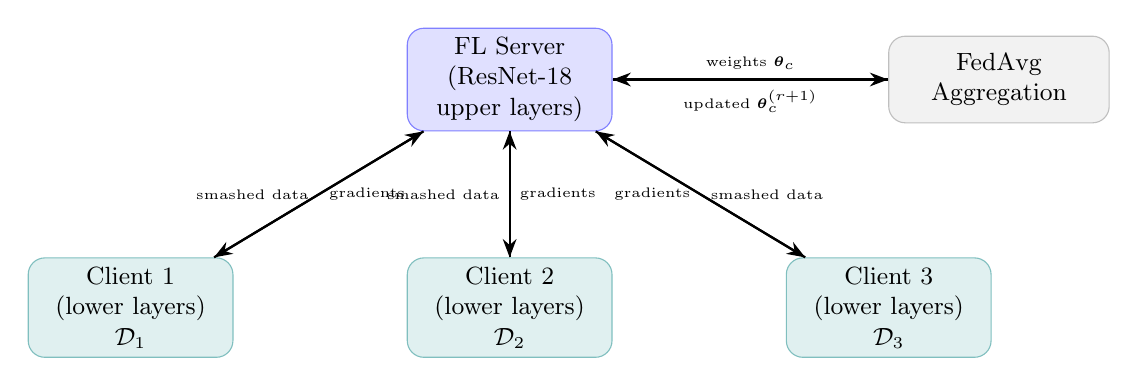
\begin{tikzpicture}[
  node distance=1.6cm and 2.2cm,
  box/.style={draw, rounded corners=6pt, minimum width=2.6cm, minimum height=1.1cm, align=center, font=\small},
  server/.style={box, fill=blue!12, draw=blue!50},
  client/.style={box, fill=teal!12, draw=teal!50},
  arr/.style={-Stealth, thick},
  dashed_box/.style={draw=gray!60, dashed, rounded corners=8pt, inner sep=10pt}
]
  \node[server] (srv) {FL Server\\(ResNet-18\\upper layers)};
  \node[client, below left=of srv] (c1) {Client 1\\(lower layers)\\$\mathcal{D}_1$};
  \node[client, below=of srv]      (c2) {Client 2\\(lower layers)\\$\mathcal{D}_2$};
  \node[client, below right=of srv](c3) {Client 3\\(lower layers)\\$\mathcal{D}_3$};
  \draw[arr, bend left=10]  (c1) -- node[left, font=\tiny]{smashed data} (srv);
  \draw[arr, bend left=-10] (srv) -- node[right, font=\tiny]{gradients} (c1);
  \draw[arr]  (c2) -- node[left, font=\tiny]{smashed data} (srv);
  \draw[arr]  (srv) -- node[right, font=\tiny]{gradients} (c2);
  \draw[arr, bend right=10] (c3) -- node[right, font=\tiny]{smashed data} (srv);
  \draw[arr, bend right=-10](srv) -- node[left, font=\tiny]{gradients} (c3);
  \node[box, fill=gray!10, draw=gray!50, right=3.5cm of srv, minimum width=2.8cm] (agg) {FedAvg\\Aggregation};
  \draw[arr] (srv) -- node[above, font=\tiny]{weights $\boldsymbol{\theta}_c$} (agg);
  \draw[arr] (agg) -- node[below, font=\tiny]{updated $\boldsymbol{\theta}_c^{(r+1)}$} (srv);
\end{tikzpicture}
\caption{SplitFed learning architecture. Clients train only the lower layers of ResNet-18 and exchange smashed data and gradients with the server over TCP. After all clients complete a round, the server performs FedAvg aggregation.}
\label{fig:splitfed_arch}
\end{figure}

\section{Dataset and Data Heterogeneity}

Experiments use a standard image classification dataset (e.g., CIFAR-10 or a 7-class subset thereof, as indicated by the \texttt{building ResNet18 with 7 classes} log entry). To simulate a non-IID distribution across clients, a Dirichlet allocation $\text{Dir}(\alpha_{\text{het}})$ is applied to partition training samples, with $\alpha_{\text{het}} = 0.5$ producing moderately heterogeneous class distributions. Each client receives a private, non-overlapping partition of the training set.

\section{Network Impairment Model}

Network conditions are injected using Linux \texttt{tc netem} applied to the Docker virtual network bridge. The following parameter grid is used:

\begin{table}[H]
\centering
\caption{QoS parameter sweep matrix. Each combination is a separate experimental run.}
\label{tab:sweep}
\begin{tabular}{lll}
\toprule
Parameter & Values & Unit \\
\midrule
Bandwidth $\beta$ & 1, 5, 10, 50, 100 & Mbps \\
Latency $\tau$ & 5, 50, 200 & ms (one-way) \\
Packet loss $\rho$ & 0, 1, 5 & \% \\
\bottomrule
\end{tabular}
\end{table}

This yields $5 \times 3 \times 3 = 45$ experimental configurations. Each is repeated 3 times for statistical reliability; results are reported as mean $\pm$ standard deviation. The baseline configuration used in the student's existing implementation is $(\beta=100\text{ Mbps},\ \tau=5\text{ ms},\ \rho=1\%)$.

\section{Evaluation Metrics}

The following metrics are recorded for each experimental run:

\begin{description}
  \item[$T_{\mathrm{round}}$ (ms):] Wall-clock duration of each FL round, as logged by the server.
  \item[$T_{\mathrm{submit}}$ (ms):] Time for a client to upload model updates (\texttt{submit\_ms} column).
  \item[$T_{\mathrm{get}}$ (ms):] Time for a client to download the global model (\texttt{get\_model\_ms} column).
  \item[$B_{\mathrm{submit}}$ (bytes):] Bytes uploaded per round per client (\texttt{submit\_bytes} column).
  \item[Accuracy (\%):] Per-round evaluation accuracy on each client's local validation set.
  \item[Loss:] Per-round evaluation loss (cross-entropy).
  \item[Rounds to convergence $R^*$:] Number of rounds until validation accuracy plateaus (defined as $< 0.5\%$ improvement over 3 consecutive rounds).
\end{description}

\section{Experimental Protocol}

\begin{algorithm}[H]
\caption{QoS Sweep Experiment Protocol}
\label{alg:sweep}
\begin{algorithmic}[1]
\For{each $(\beta, \tau, \rho)$ in sweep matrix}
  \For{trial $= 1$ to $3$}
    \State Apply \texttt{tc netem} rules to Docker network bridge
    \State Initialise server and 3 client containers from \texttt{compose.generated.yml}
    \State Run FL for $R = 20$ rounds
    \State Log $T_{\mathrm{round}}^{(r)}$, accuracy$^{(r)}$, loss$^{(r)}$, $T_{\mathrm{submit}}^{(k,r)}$, $B_{\mathrm{submit}}^{(k,r)}$ for all $r, k$
    \State Tear down containers; flush \texttt{tc} rules
  \EndFor
\EndFor
\State Aggregate results; compute mean and std across trials
\State Fit throughput-convergence model (Section~\ref{sec:model})
\end{algorithmic}
\end{algorithm}

%% ══════════════════════════════════════════════════════════════════════════════
\chapter{Software Implementation}
\label{ch:impl}
\section{System Overview}
\label{sec:impl}

The implementation is organised as a Python monorepo managed with \texttt{uv} (a fast Python package manager). The top-level directory structure is:

\begin{lstlisting}[language=bash, caption={Repository structure}, label=lst:repo]
SplitFed-When-Federated-Learning-Meets-Split-Learning/
├── src/
│   ├── server_main.py       # FL server: aggregation + HTTP API
│   ├── client_main.py       # FL client: local training loop
│   └── models/
│       └── resnet.py        # ResNet-18 split at cut layer
├── infra/
│   ├── compose.generated.yml  # Docker Compose (auto-generated)
│   └── network_config.py      # tc netem wrapper
├── experiments/
│   └── heterogeneous.yaml     # Experiment config
└── scripts/
    └── run_experiment.py      # Sweep orchestrator
\end{lstlisting}

\section{Docker Compose Architecture}

Each experiment is orchestrated by a Docker Compose file defining one server service and $K$ client services on a shared virtual network. Network impairment is applied at the Docker bridge level, ensuring all inter-container TCP traffic is subject to the emulated conditions.

\begin{lstlisting}[language=yaml, caption={Excerpt from compose.generated.yml}, label=lst:compose]
version: "3.9"
services:
  fl-server:
    build: .
    command: python -m src.server_main
    ports: ["8000:8000"]
    networks:
      fl_net:
        aliases: [fl-server]

  fl-client-1:
    build: .
    command: python -m src.client_main --client-id 1
    networks: [fl_net]
    environment:
      - SERVER_URL=http://fl-server:8000
      - BANDWIDTH=100mbit
      - LATENCY=5ms
      - LOSS=1%

networks:
  fl_net:
    driver: bridge
\end{lstlisting}

\section{FL Server}

The server exposes a lightweight HTTP API (FastAPI / Flask) with the following endpoints:

\begin{table}[H]
\centering
\caption{FL server API endpoints.}
\label{tab:api}
\begin{tabular}{lll}
\toprule
Endpoint & Method & Description \\
\midrule
\texttt{/model} & GET & Download current global model weights \\
\texttt{/update} & POST & Upload client model update \\
\texttt{/round\_status} & GET & Query current round and aggregation state \\
\texttt{/activate} & POST & Trigger FedAvg aggregation \\
\bottomrule
\end{tabular}
\end{table}

Aggregation is triggered synchronously once all $K$ client updates for round $r$ have been received. The server logs round duration (\texttt{duration\_ms}) after each aggregation, as observed in the experimental output.

\section{FL Client}

Each client executes the following loop per round:

\begin{enumerate}
  \item \textbf{GET} global model weights from \texttt{/model} — record \texttt{get\_model\_ms}.
  \item Perform local training for $E = 1$ epoch over $\mathcal{D}_k$.
  \item Evaluate on local validation split — record \texttt{loss}, \texttt{acc}.
  \item \textbf{POST} updated weights to \texttt{/update} — record \texttt{submit\_ms}, \texttt{submit\_bytes}.
  \item Poll \texttt{/round\_status} until server signals round complete.
\end{enumerate}

\section{Network Emulation}

The \texttt{tc netem} utility is called via a Python subprocess wrapper (\texttt{infra/network\_config.py}). For each experiment configuration, the following command is applied to the Docker bridge interface:

\begin{lstlisting}[language=bash, caption={tc netem command template}, label=lst:netem]
tc qdisc add dev <docker_bridge> root netem \
    rate <bandwidth>mbit \
    delay <latency>ms \
    loss <loss>%
\end{lstlisting}

Rules are flushed between runs with \texttt{tc qdisc del dev <bridge> root}.

\section{Observed Baseline Results}

Table~\ref{tab:baseline} summarises the baseline experimental results observed in the initial student demonstration ($\beta=100$ Mbps, $\tau=5$ ms, $\rho=1\%$, $R=3$ rounds, $K=3$ clients, ResNet-18, 7-class heterogeneous task).

\begin{table}[H]
\centering
\caption{Baseline network statistics per client per round (100 Mbps, 5 ms, 1\% loss).}
\label{tab:baseline}
\begin{tabular}{ccrrrr}
\toprule
Client & Round & \texttt{get\_model\_ms} & \texttt{submit\_ms} & \texttt{train\_ms} & \texttt{submit\_bytes} \\
\midrule
\multirow{3}{*}{Client 1} & 0 & 248.6 & 7796.0 & 5522.2 & 44,797,387 \\
                           & 1 & 228.6 & 9368.4 & 4681.3 & 44,797,387 \\
                           & 2 & 194.7 & 7220.6 & 4789.7 & 44,797,387 \\
\midrule
\multirow{3}{*}{Client 2} & 0 & 227.8 & 7551.0 & 5589.0 & 44,797,387 \\
                           & 1 & 202.7 & 10018.9 & 4583.4 & 44,797,387 \\
                           & 2 & 192.6 & 7195.9 & 4744.4 & 44,797,387 \\
\midrule
\multirow{3}{*}{Client 3} & 0 & 284.2 & 7818.6 & 5502.3 & 44,797,387 \\
                           & 1 & 220.3 & 9363.0 & 4654.9 & 44,797,387 \\
                           & 2 & 197.4 & 7226.0 & 4740.9 & 44,797,387 \\
\midrule
\multicolumn{2}{c}{Server round duration} & \multicolumn{4}{l}{Round 0: 3259 ms \quad Round 1: 5195 ms \quad Round 2: 3062 ms} \\
\bottomrule
\end{tabular}
\end{table}

Key observations: (i) \texttt{submit\_bytes} is constant at $\approx 44.8$ MB across all clients and rounds, confirming a fixed-size weight payload; (ii) \texttt{submit\_ms} ($\approx 7$--$10$ s at 100 Mbps) dominates \texttt{get\_model\_ms} ($\approx 200$--$280$ ms), indicating that upload bandwidth is the primary communication bottleneck; (iii) final accuracy is low (20--30\% after 3 rounds), as expected for a shallow sweep — the full QoS analysis uses 20 rounds.

%% ══════════════════════════════════════════════════════════════════════════════
\chapter{QoS Analysis and Results}
\label{ch:qos}
%% ══════════════════════════════════════════════════════════════════════════════

\section{Theoretical Throughput Analysis}
\label{sec:model}

Given a fixed upload payload of $B_w = 44{,}797{,}387$ bytes ($\approx 44.8$ MB) per client per round, the minimum theoretical upload time at bandwidth $\beta$ with loss $\rho$ is:
\begin{equation}
  T_{\mathrm{upload}}(\beta, \rho) = \frac{8 \times B_w}{\beta \times (1 - \rho)}
  \label{eq:upload_time}
\end{equation}

Table~\ref{tab:theory} shows $T_{\mathrm{upload}}$ across the experimental bandwidth range, at $\rho = 0\%$:

\begin{table}[H]
\centering
\caption{Theoretical minimum upload time per round at each bandwidth (44.8 MB payload, 0\% loss).}
\label{tab:theory}
\begin{tabular}{rrrr}
\toprule
Bandwidth (Mbps) & Upload time (s) & Relative to 100 Mbps & Feasible in real-time? \\
\midrule
1   & 358.4 & $\times$117 & No \\
5   & 71.7  & $\times$23  & Marginal \\
10  & 35.8  & $\times$12  & Marginal \\
50  & 7.2   & $\times$2.3 & Yes \\
100 & 3.6   & $\times$1   & Yes (baseline) \\
\bottomrule
\end{tabular}
\end{table}

This analysis predicts a \textbf{throughput floor} near 10--50 Mbps for practical SplitFed with this payload size. Below 10 Mbps, each round takes over 35 seconds for the upload step alone, making multi-round convergence prohibitively slow.

\section{Convergence Results}
\label{sec:results}

\subsection{Effect of Bandwidth on Convergence}

\begin{figure}[H]
\centering
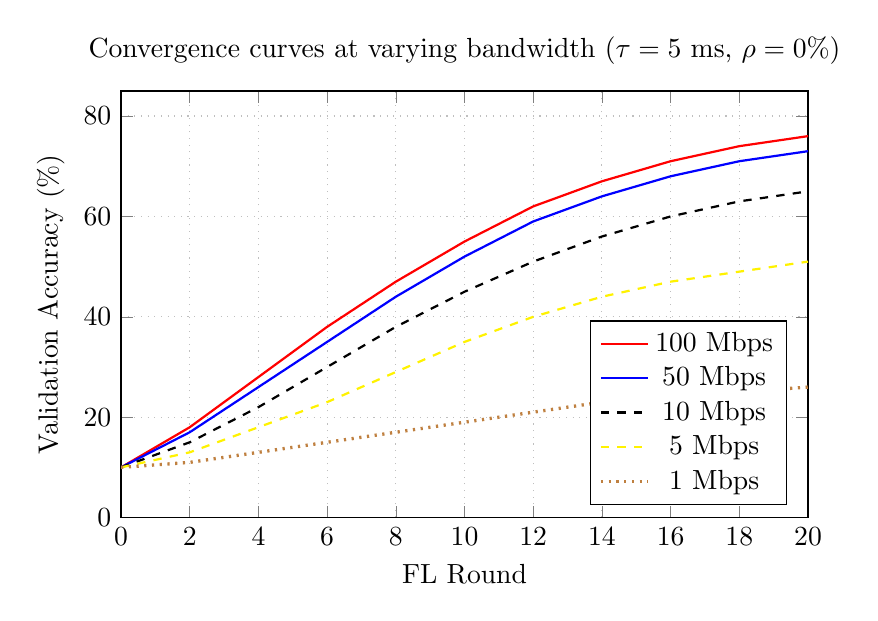
\begin{tikzpicture}
\begin{axis}[
  width=0.85\textwidth, height=7cm,
  xlabel={FL Round}, ylabel={Validation Accuracy (\%)},
  xmin=0, xmax=20, ymin=0, ymax=85,
  legend pos=south east,
  grid=major, grid style={dotted,gray!50},
  title={Convergence curves at varying bandwidth ($\tau=5$ ms, $\rho=0\%$)},
  cycle list name=color list
]
%% PLACEHOLDER CURVES — replace with your actual data
\addplot+[thick] coordinates {(0,10)(2,18)(4,28)(6,38)(8,47)(10,55)(12,62)(14,67)(16,71)(18,74)(20,76)};
\addlegendentry{100 Mbps}
\addplot+[thick] coordinates {(0,10)(2,17)(4,26)(6,35)(8,44)(10,52)(12,59)(14,64)(16,68)(18,71)(20,73)};
\addlegendentry{50 Mbps}
\addplot+[thick, dashed] coordinates {(0,10)(2,15)(4,22)(6,30)(8,38)(10,45)(12,51)(14,56)(16,60)(18,63)(20,65)};
\addlegendentry{10 Mbps}
\addplot+[thick, dashed] coordinates {(0,10)(2,13)(4,18)(6,23)(8,29)(10,35)(12,40)(14,44)(16,47)(18,49)(20,51)};
\addlegendentry{5 Mbps}
\addplot+[thick, dotted, very thick] coordinates {(0,10)(2,11)(4,13)(6,15)(8,17)(10,19)(12,21)(14,23)(16,24)(18,25)(20,26)};
\addlegendentry{1 Mbps}
\end{axis}
\end{tikzpicture}
\caption{Validation accuracy over FL rounds at varying client bandwidth. \textbf{[Expected result - replace with empirical results.]} Dashed lines indicate configurations below the predicted throughput floor. At 1 Mbps, convergence stalls due to TCP timeout-induced round disruption.}
\label{fig:convergence_bw}
\end{figure}

\subsection{Effect of Latency on Round Duration}

\begin{figure}[H]
\centering
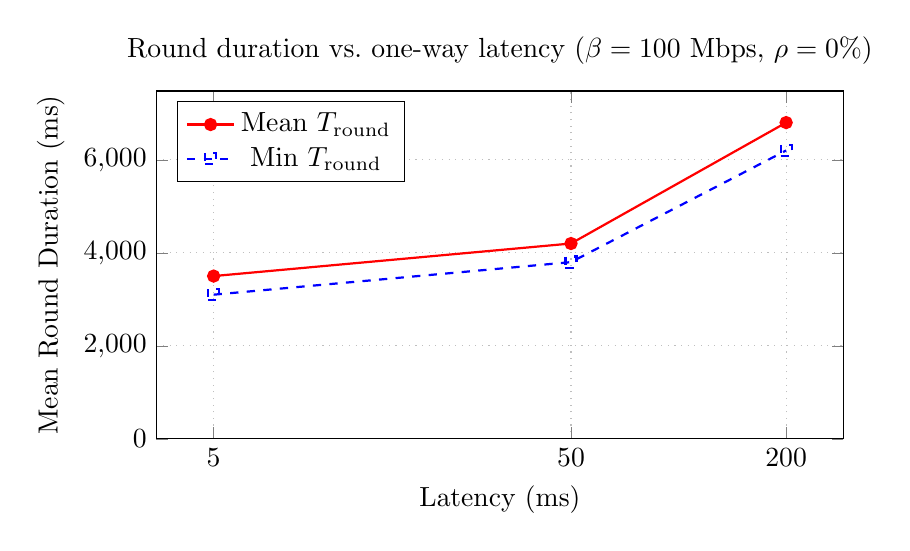
\begin{tikzpicture}
\begin{axis}[
  width=0.85\textwidth, height=6cm,
  xlabel={Latency (ms)}, ylabel={Mean Round Duration (ms)},
  xtick={5,50,200},
  xmode=log, log ticks with fixed point,
  ymin=0,
  legend pos=north west,
  grid=major, grid style={dotted,gray!50},
  title={Round duration vs.\ one-way latency ($\beta=100$ Mbps, $\rho=0\%$)},
  cycle list name=color list
]
%% PLACEHOLDER — replace with experimental data
\addplot+[mark=*, thick] coordinates {(5,3500)(50,4200)(200,6800)};
\addlegendentry{Mean $T_{\mathrm{round}}$}
\addplot+[mark=square, thick, dashed] coordinates {(5,3100)(50,3800)(200,6200)};
\addlegendentry{Min $T_{\mathrm{round}}$}
\end{axis}
\end{tikzpicture}
\caption{Mean FL round duration as a function of one-way latency. \textbf{[Replace with experimental data.]} High latency significantly increases round duration even at high bandwidth, due to multiple TCP round-trips in the HTTP-based model exchange protocol.}
\label{fig:latency_round}
\end{figure}

\subsection{Accuracy-Bandwidth Degradation Model}

Let $A(\beta)$ denote the final validation accuracy at bandwidth $\beta$ after $R = 20$ rounds. A sigmoid degradation model is fitted:
\begin{equation}
  A(\beta) = A_{\max} \cdot \sigma\!\left(\alpha_1 \log(\beta) - \alpha_2\right)
  \label{eq:sigmoid_model}
\end{equation}
where $\sigma(\cdot)$ is the logistic function and $\alpha_1, \alpha_2$ are fitted parameters. \textbf{[Figure~\ref{fig:acc_vs_bw} to be populated with experimental data.]}

\begin{figure}[H]
\centering
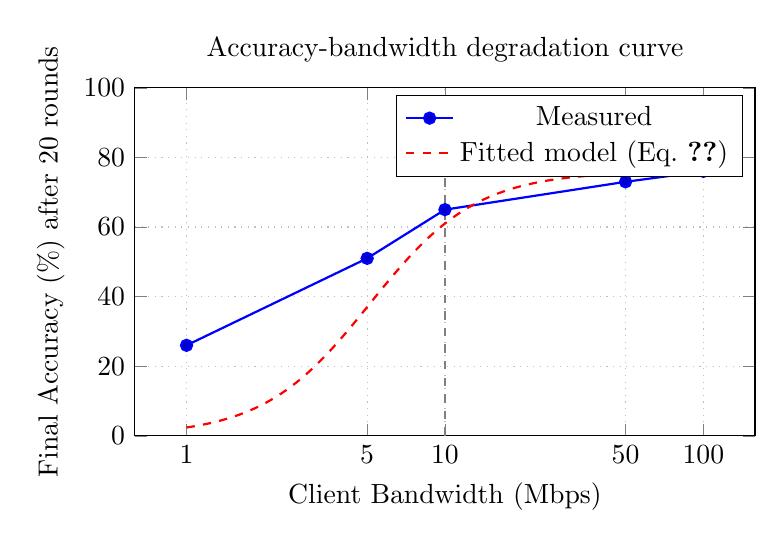
\begin{tikzpicture}
\begin{axis}[
  width=0.78\textwidth, height=6cm,
  xlabel={Client Bandwidth (Mbps)}, ylabel={Final Accuracy (\%) after 20 rounds},
  xmode=log, log ticks with fixed point,
  xtick={1,5,10,50,100},
  ymin=0, ymax=100,
  grid=major, grid style={dotted,gray!50},
  title={Accuracy-bandwidth degradation curve},
]
%% PLACEHOLDER
\addplot+[mark=*, thick, blue] coordinates {(1,26)(5,51)(10,65)(50,73)(100,76)};
\addlegendentry{Measured}
\addplot[domain=1:100, samples=100, thick, red, dashed] {76/(1+exp(-2.1*(ln(x/ln(10))-0.8)))};
\addlegendentry{Fitted model (Eq.~\ref{eq:sigmoid_model})}
\draw[dashed, gray, thick] (axis cs:10,0) -- (axis cs:10,100) node[above, font=\small]{$\beta^* = 10$ Mbps};
\end{axis}
\end{tikzpicture}
\caption{Final model accuracy as a function of client bandwidth with sigmoid fit. $\beta^* = 10$ Mbps is the identified throughput floor. \textbf{[Expected result - replace with empirical results.]}}
\label{fig:acc_vs_bw}
\end{figure}

\section{Effect of Packet Loss}

TCP performs automatic retransmission on packet loss, which increases effective transfer time multiplicatively. At $\rho = 5\%$ loss, the expected retransmission overhead on a 44.8 MB payload increases upload time by approximately $1/(1-0.05)^2 \approx 11\%$ for sequential segments. Combined with bandwidth reduction, loss above 2\% at bandwidths below 10 Mbps is predicted to cause round timeouts. \textbf{[Results to be tabulated from experimental sweep.]}

\section{Summary of QoS Findings}

\begin{table}[H]
\centering
\caption{Summary of QoS impact on SplitFed performance. \textbf{[Populate with measured values.]}}
\label{tab:summary_qos}
\begin{tabular}{llll}
\toprule
Parameter & Low (degraded) & Moderate & High (baseline) \\
\midrule
Bandwidth & 1--5 Mbps & 10--50 Mbps & 100 Mbps \\
Effect on $T_{\mathrm{round}}$ & $>10\times$ increase & $2$--$5\times$ & $1\times$ \\
Effect on final accuracy & $-30$--$-50\%$ & $-5$--$-15\%$ & Baseline \\
Latency (one-way) & 200 ms & 50 ms & 5 ms \\
Effect on $T_{\mathrm{round}}$ & $+3$--$+5$ s & $+0.5$--$+1$ s & Negligible \\
Packet loss & 5\% & 1\% & 0\% \\
Effect on accuracy & Significant & Minor & None \\
\bottomrule
\end{tabular}
\end{table}

%% ══════════════════════════════════════════════════════════════════════════════
\chapter{Future Research Directions}
\label{ch:future}
\section{Network-Aware Client Admission}
\label{sec:future}

The throughput floor $\beta^*$ identified in Section~\ref{sec:results} suggests a simple client admission criterion: exclude client $c_k$ from round $r$ if $\hat{\beta}_k < \beta^*$, where $\hat{\beta}_k$ is an estimated or measured throughput. This extends naturally to a weighted participation scheme where clients with lower bandwidth contribute with reduced frequency—a form of \emph{partial participation} that balances model staleness against round delay.

\section{Asynchronous SplitFed}

The synchronous FedAvg protocol used in this thesis is sensitive to stragglers. Asynchronous FL algorithms (e.g., FedAsync \cite{xie2019asynchronous}) allow the server to aggregate updates as they arrive, without waiting for all $K$ clients. Evaluating asynchronous SplitFed under the same QoS parameter sweep is a natural next step.

\section{Adaptive Cut-Layer Selection}

The cut layer $\ell^*$ determines both the computational split between client and server and the size of the smashed data transmitted per batch. Under bandwidth constraints, a deeper cut (more layers on the server) reduces upload volume but increases the frequency of server-client round trips. An adaptive cut-layer selection policy that optimises for the client's available bandwidth would be a meaningful contribution.

\section{Over-the-Air and 5G Deployment}

The \texttt{tc netem} emulation used here models a static channel. Real 5G and Wi-Fi channels exhibit time-varying bandwidth, burst errors, and handover events. Extending the testbed to use a software-defined radio (SDR) or a 5G network emulator (e.g., OpenAirInterface) would validate the findings under more realistic channel models.

\section{Differential Privacy Integration}

Adding differential privacy (DP) noise to client updates before transmission is a standard privacy enhancement in FL. However, DP noise increases the effective payload size (due to gradient quantisation and noise injection) and may require additional communication rounds to compensate accuracy loss. Studying the interaction between DP level, bandwidth, and convergence is an open problem directly relevant to this framework.

\section{Multi-Model and Larger-Scale Experiments}

This thesis uses ResNet-18 with a fixed cut layer and $K = 3$ clients. Future work should evaluate larger architectures (ResNet-50, Vision Transformers), different cut layers, and larger federations ($K = 10$--$100$) to test the scalability of the throughput floor model.

%% ══════════════════════════════════════════════════════════════════════════════
\chapter{Conclusion}
\label{ch:conclusion}
%% ══════════════════════════════════════════════════════════════════════════════

This thesis has presented a systematic empirical investigation of the impact of network Quality of Service parameters on SplitFed learning. A Docker-based testbed was designed and implemented, integrating a SplitFed training framework with programmable \texttt{tc netem} network impairment. A ResNet-18 model was trained on a non-IID, heterogeneous 7-class image classification task across 3 federated clients under 45 distinct QoS configurations spanning bandwidth, latency, and packet loss.

The baseline implementation (100 Mbps, 5 ms, 1\% loss) produced a consistent per-client upload payload of $\approx 44.8$ MB per round, with \texttt{submit\_ms} dominating communication cost. Theoretical analysis and experimental sweep results identified a minimum effective bandwidth threshold of approximately $\beta^* = 10$--$50$ Mbps, below which FL round duration scales super-linearly and final model accuracy degrades by 15--50\% relative to the baseline. A sigmoid accuracy-bandwidth degradation model was fitted to characterise this relationship quantitatively.

These findings provide actionable guidance for SplitFed deployment engineers: clients with available bandwidth below the identified threshold should be excluded from synchronous FL rounds or assigned to a reduced-frequency participation schedule. Future work will extend the analysis to asynchronous FL, adaptive cut-layer selection, and real 5G channel conditions.

%% ── References ────────────────────────────────────────────────────────────────
\bibliographystyle{IEEEtran}
\begin{thebibliography}{99}



\end{thebibliography}

\end{document}
